\documentclass[
]{beamer}
\usepackage[czech]{babel}
\usepackage[utf8]{inputenc}
\usepackage[T1]{fontenc}
\usepackage{booktabs}

\usetheme[
  workplace=fi,
]{MU}
\begin{document}

\title[Obhajoba diplomové práce]{Autentizační a autorizační infrastruktura pro videokonferenční prostředí}
\subtitle[Short Presentation Subtitle]{Obhajoba diplomové práce}
\author[L.\,Kotol]{Bc. Lukáš Kotol \\ 433265@mail.muni.cz}
\institute[FI MU]{Fakulta informatiky, Masarykova Univerzita}
\date{\today}
\subject{Presentation Subject}
\keywords{the, presentation, keywords}

\begin{frame}[plain]
\maketitle
\end{frame}

\section[Zadání]{Zadání}

\begin{frame}{Představení zadání}{}
Zadání diplomové práce sestávalo z vytvoření nové \structure{autentizační a autorizační infrastruktury pro videokonferenční prostředí}. 
\\
\medskip
Součástí webkonferenčního prostředí jsou služby
\structure{meetings.cesnet.cz} a \structure{Adobe Connect}.

\end{frame}

\begin{frame}{Služba meetings.cesnet.cz}

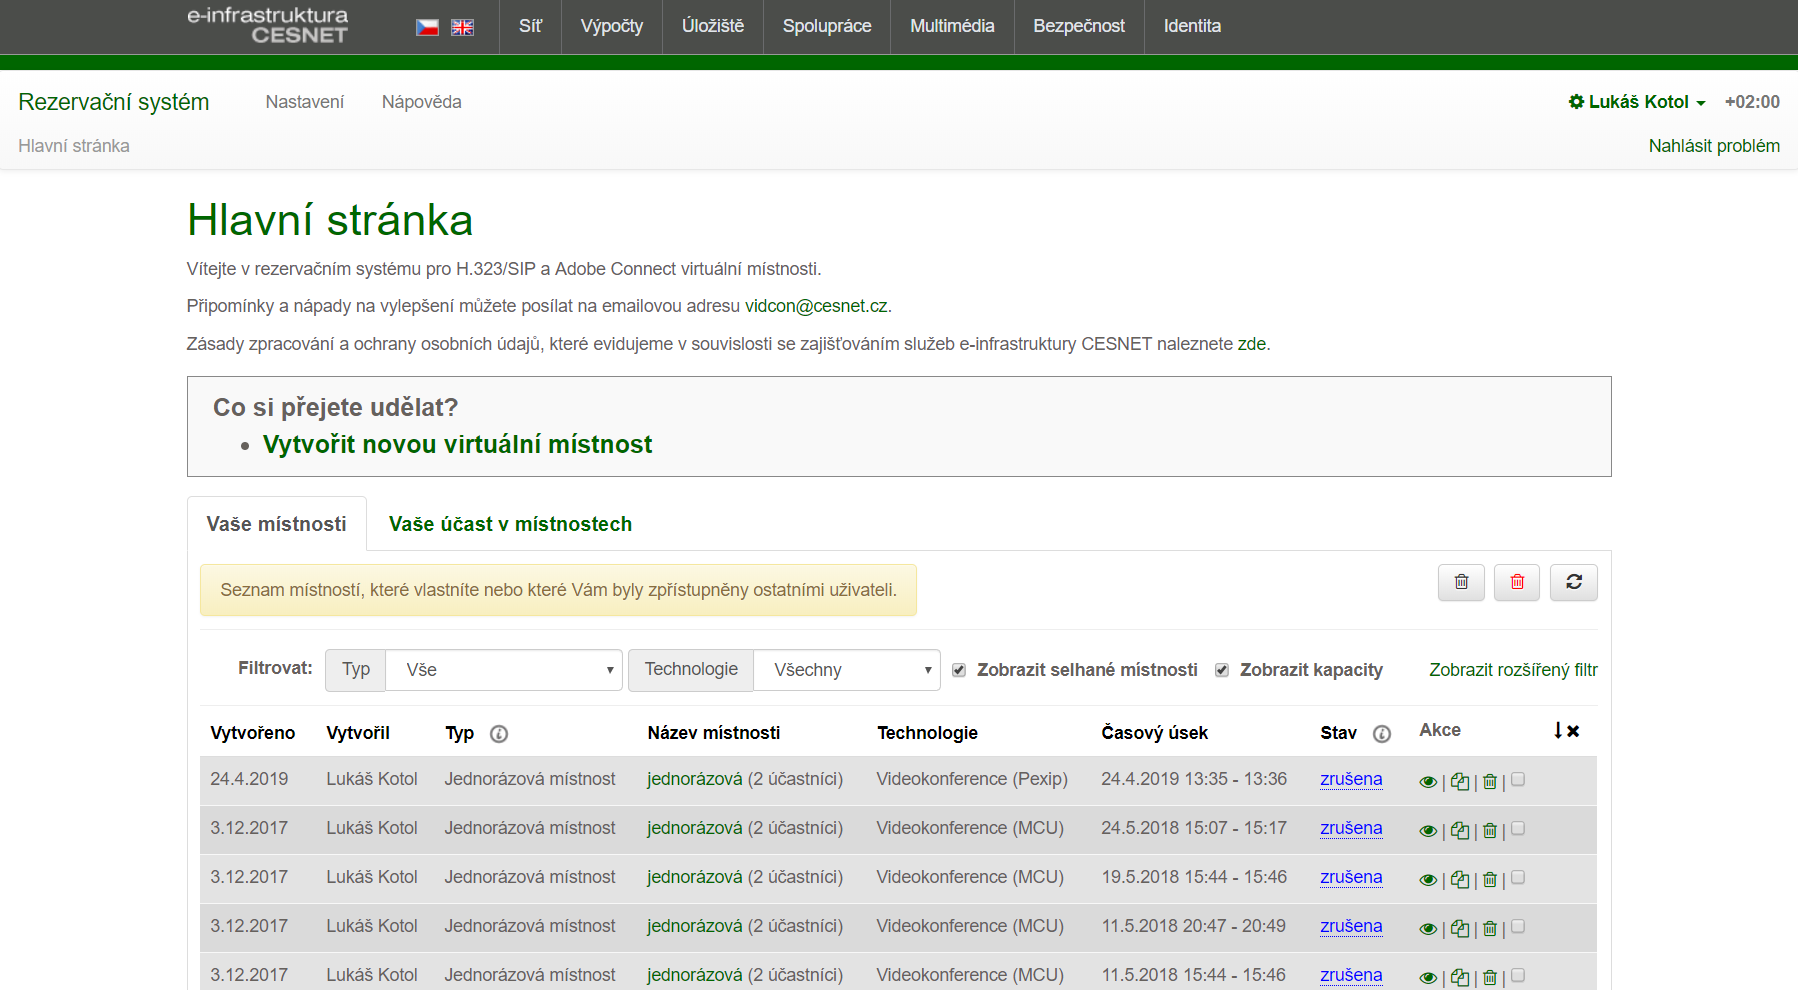
\includegraphics[width=\textwidth]{pics/rezervacni_system}
\end{frame}

\begin{frame}{Webkonferenční služba realizovaná technologií Adobe Connect}

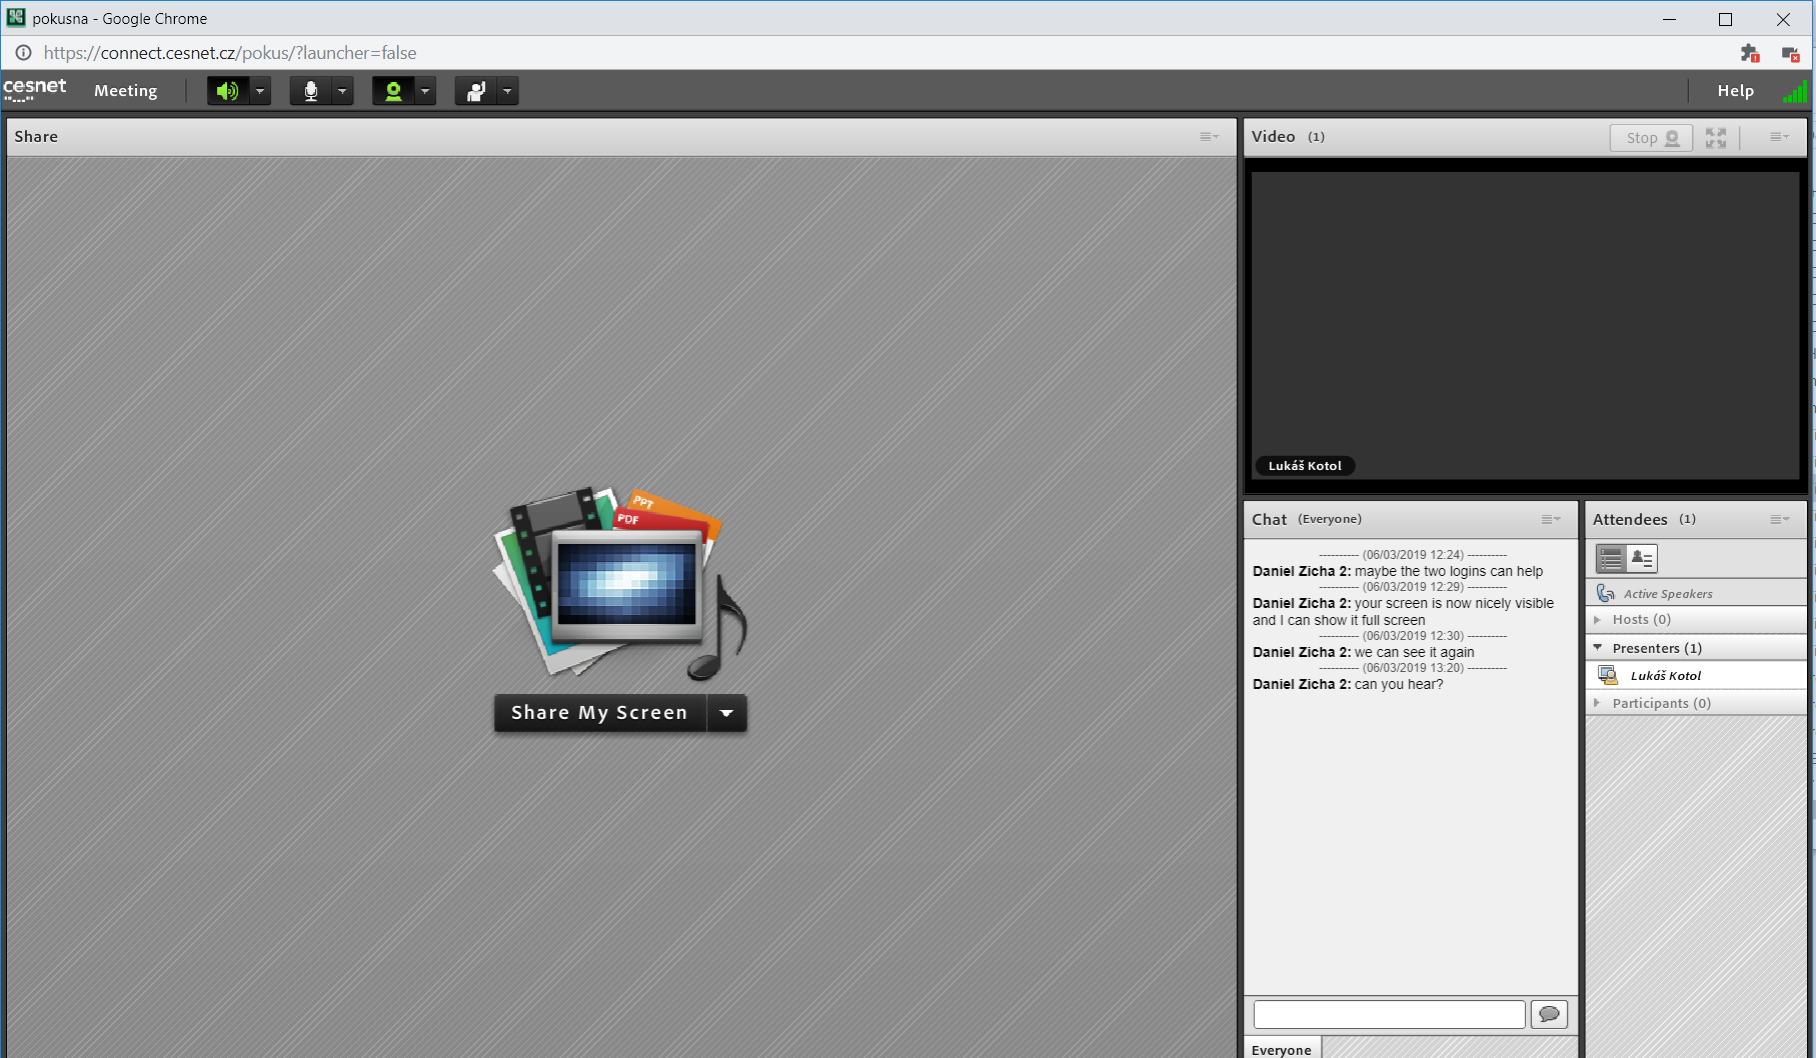
\includegraphics[width=\textwidth]{pics/adobe_connect.PNG}
\end{frame}

\begin{frame}{Specifikace zadání}
Nová autentizační a autorizační infrastruktura bude
\begin{itemize}
  \item integrována do \structure{Proxy IdP v infrastruktuře CESNETu} \cite{proxyIdpPresentation},
  \item založena na technologii \structure{OpenID Connect} \cite{oidcPresentation}.
\end{itemize}
\end{frame}

\section[Proxy Idp]{Proxy Idp}
\begin{frame}{Proxy IdP infrastruktura}
\begin{itemize}
    \item zajišťuje bezpečný přístup ke službám \structure{CESNET eInfrastruktury},
    \item umožňuje delegaci procesu autentizace a autorizace,
    \item služby a poskytovatelé identit jsou sdruženy do České akademické federace identit \structure{eduID.cz}.

\end{itemize}
\end{frame}

\section[OpenID Connect]{OpenID Connect}

\begin{frame}{OpenID Connect}
\framesubtitle{Představení protokolu}
Protokol, umožňující aplikaci verifikovat identitu uživatele na základě autentizace provedené autorizačním serverem.
\\
\medskip
Klíčové vlastnosti:
\begin{itemize}
  \item autentizační vrstva nad protokolem \structure{OAuth} \cite{rfc6749},
  \item definuje způsob získávání informací o přihlášeném uživateli,
  \item specifikuje koncové body, tzv. \structure{Endpointy}.
\end{itemize}
\end{frame}

\begin{frame}{OpenID Connect}
\framesubtitle{Schéma komunikace v protokolu}
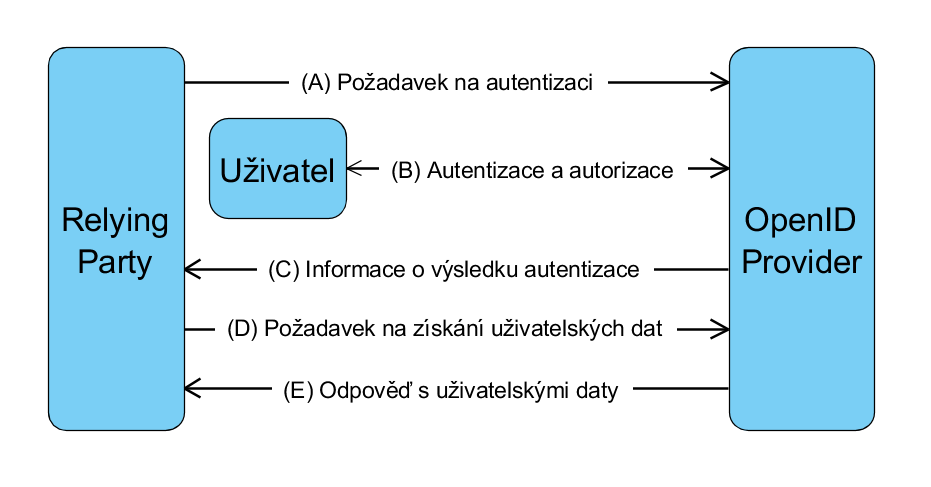
\includegraphics[width=\textwidth]{pics/diplomkaOIDC}
\end{frame}


\section[Implementace autentizační a autorizační infrastruktury]{Implementace autentizační a autorizační infrastruktury}

\begin{frame}{Vypracování diplomové práce}
\framesubtitle{Instalace a konfigurace Apache modulu pro OpenID Connect \cite{oidcConfigPresentation}}
Integrace OpenID Connect modulu do autentizační a autorizační infrastruktury sestávala z
\begin{itemize}
    \item instalace modulu \structure{mod\_auth\_openidc},
    \item registrace klienta do Proxy IdP,
    \item konfigurace modulu \structure{mod\_auth\_openidc}.
\end{itemize}
\end{frame}

\begin{frame}{Registrace klienta do Proxy IdP}

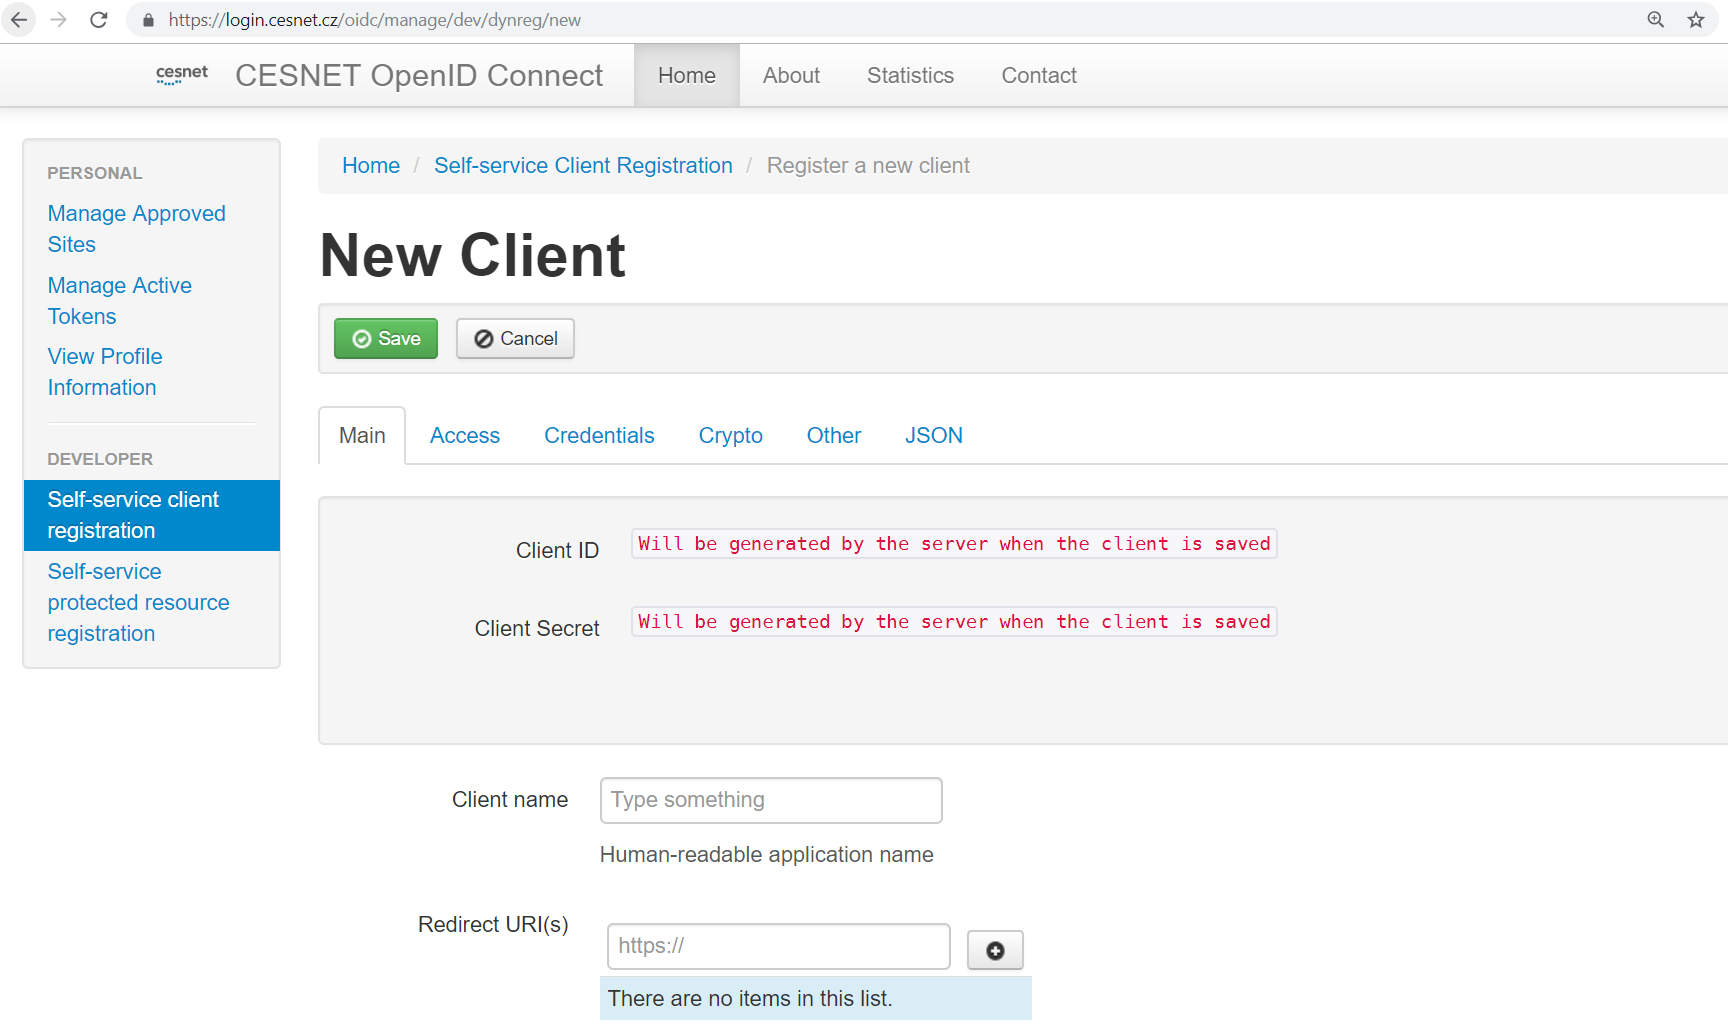
\includegraphics[width=\textwidth]{pics/oidcRegistration}
\end{frame}

\begin{frame}{Vypracování diplomové práce}
\framesubtitle{Autentizační vrstva služby Adobe Connect}
Navrhl a implementoval jsem
\begin{itemize}
    \item přemapování uživatelských atributů,
    \item logiku vytváření nových uživatelů ve službě Adobe Connect.
\end{itemize}
\end{frame}

\begin{frame}{Vypracování diplomové práce}
\framesubtitle{Autentizační a autorizační vrstva služby meetings.cesnet.cz}
Navrhl a implementoval jsem
\begin{itemize}
    \item novou autentizační a autorizační logiku na serveru \structure{shongo-auth.cesnet.cz},
    \item odstranění závislosti na webové službě \structure{Perun} \cite{perunPresentation},
    \item adaptaci služby \structure{meetings.cesnet.cz} na novou autentizační a autorizační vrstvu.
\end{itemize}
\end{frame}

\begin{frame}{Schéma komunikace při zpracování autentizačního požadavku ve stávající infrastruktuře}

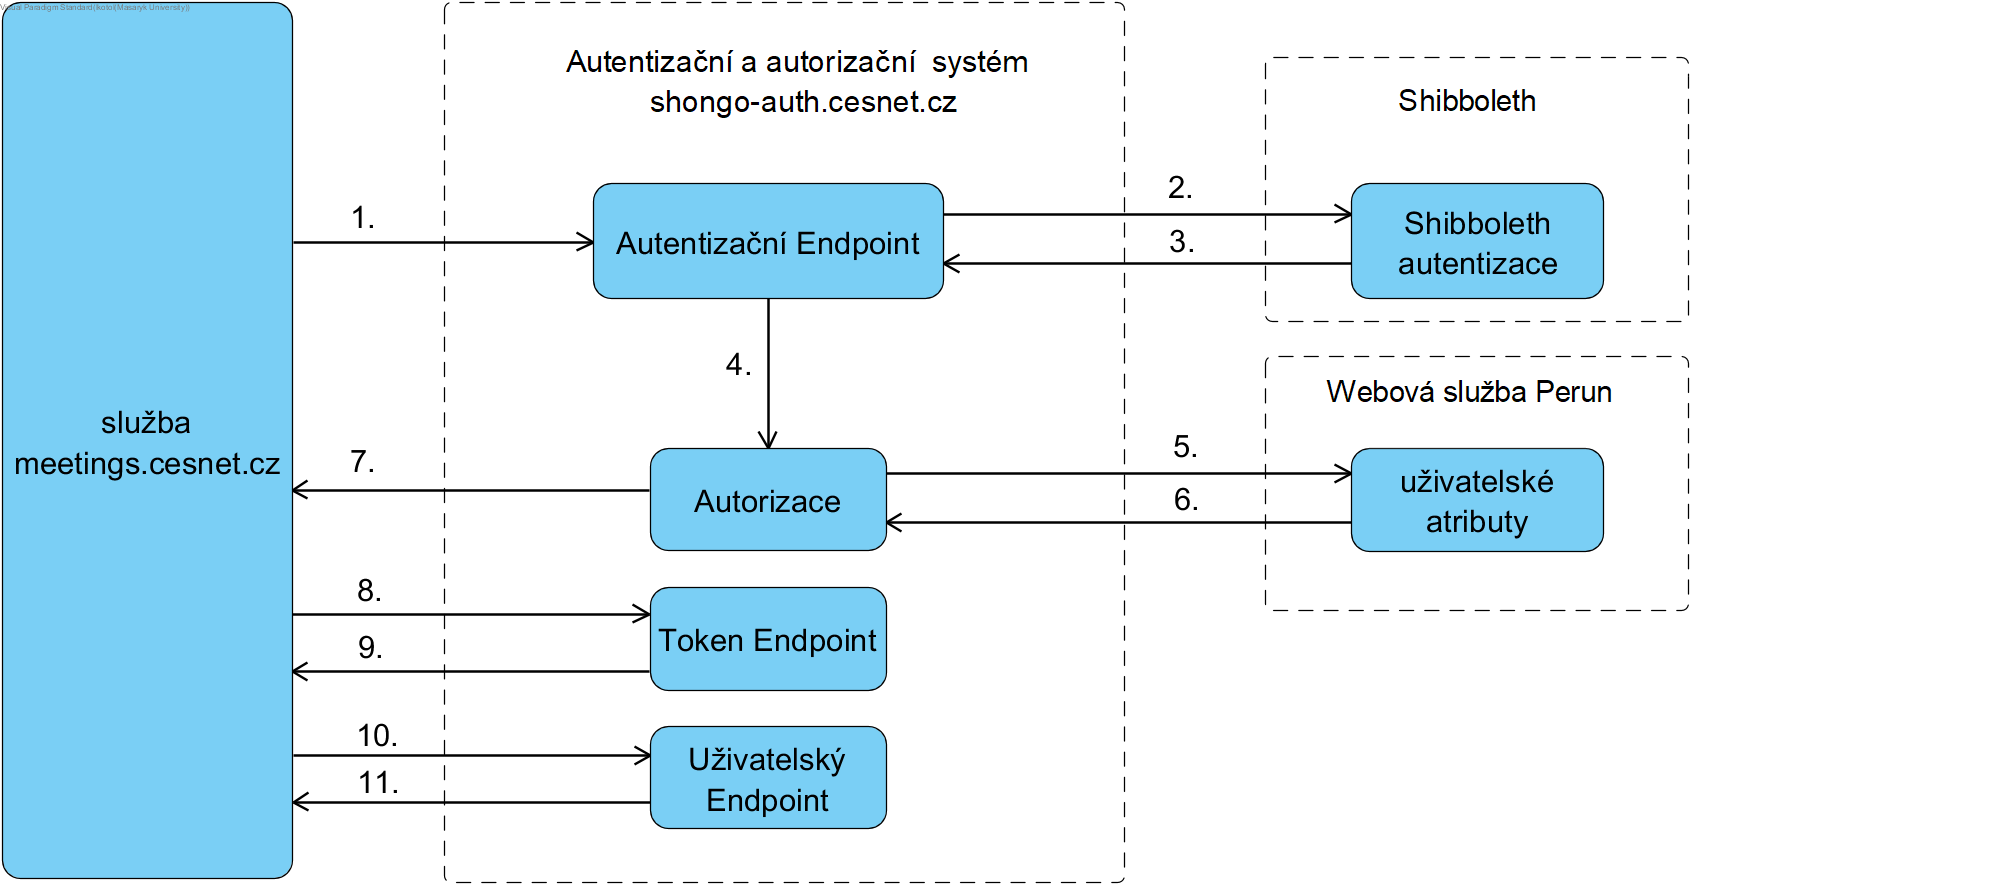
\includegraphics[width=\textwidth]{pics/meetings-perun-obhajoba.png}
\end{frame}

\begin{frame}{Vypracování diplomové práce}
\framesubtitle{Implementace na straně serveru shongo-auth.cesnet.cz}

Autentizační a autorizační komponenta mezi poskytovatelem \structure{OpenID Connect} a službou \structure{meetings.cesnet.cz}.
\\
\medskip
Zde jsem navrhl a implementoval 
\begin{itemize}
    \item delegování autentizace na autorizační server OpenID Connect,
    \item získání a zpracovaní uživatelských atributů po autentizaci,
    \item autorizační logiku. 
\end{itemize}
\end{frame}

\begin{frame}{Vypracování diplomové práce}
\framesubtitle{Odstranění závislosti na webové službě Perun}
Perun je služba určená pro správu uživatelů v eInfrastruktuře. 
\\
\medskip
Implementoval jsem algoritmus, který prostřednictvím jednorázového využití \structure{webové služby Perun}  
\begin{itemize}
    \item nahradil identifikátory uživatele,
    \item uložil dodatečné uživatelské informace do databáze služby \structure{meetings.cesnet.cz}.
\end{itemize}
\end{frame}


\begin{frame}{Vypracování diplomové práce}
\framesubtitle{Adaptace služby meetings.cesnet.cz na novou autentizační a autorizační vrstvu}
Adaptace sestávala z 

\begin{itemize}
    \item napojení na nové endpointy využívající OpenID Connect,
    \item využití zpracovaných uživatelských informací,
    \item odstranění nepotřebných volání služby Perun.
\end{itemize}

\end{frame}

\begin{frame}{Schéma komunikace při zpracování autentizačního požadavku}

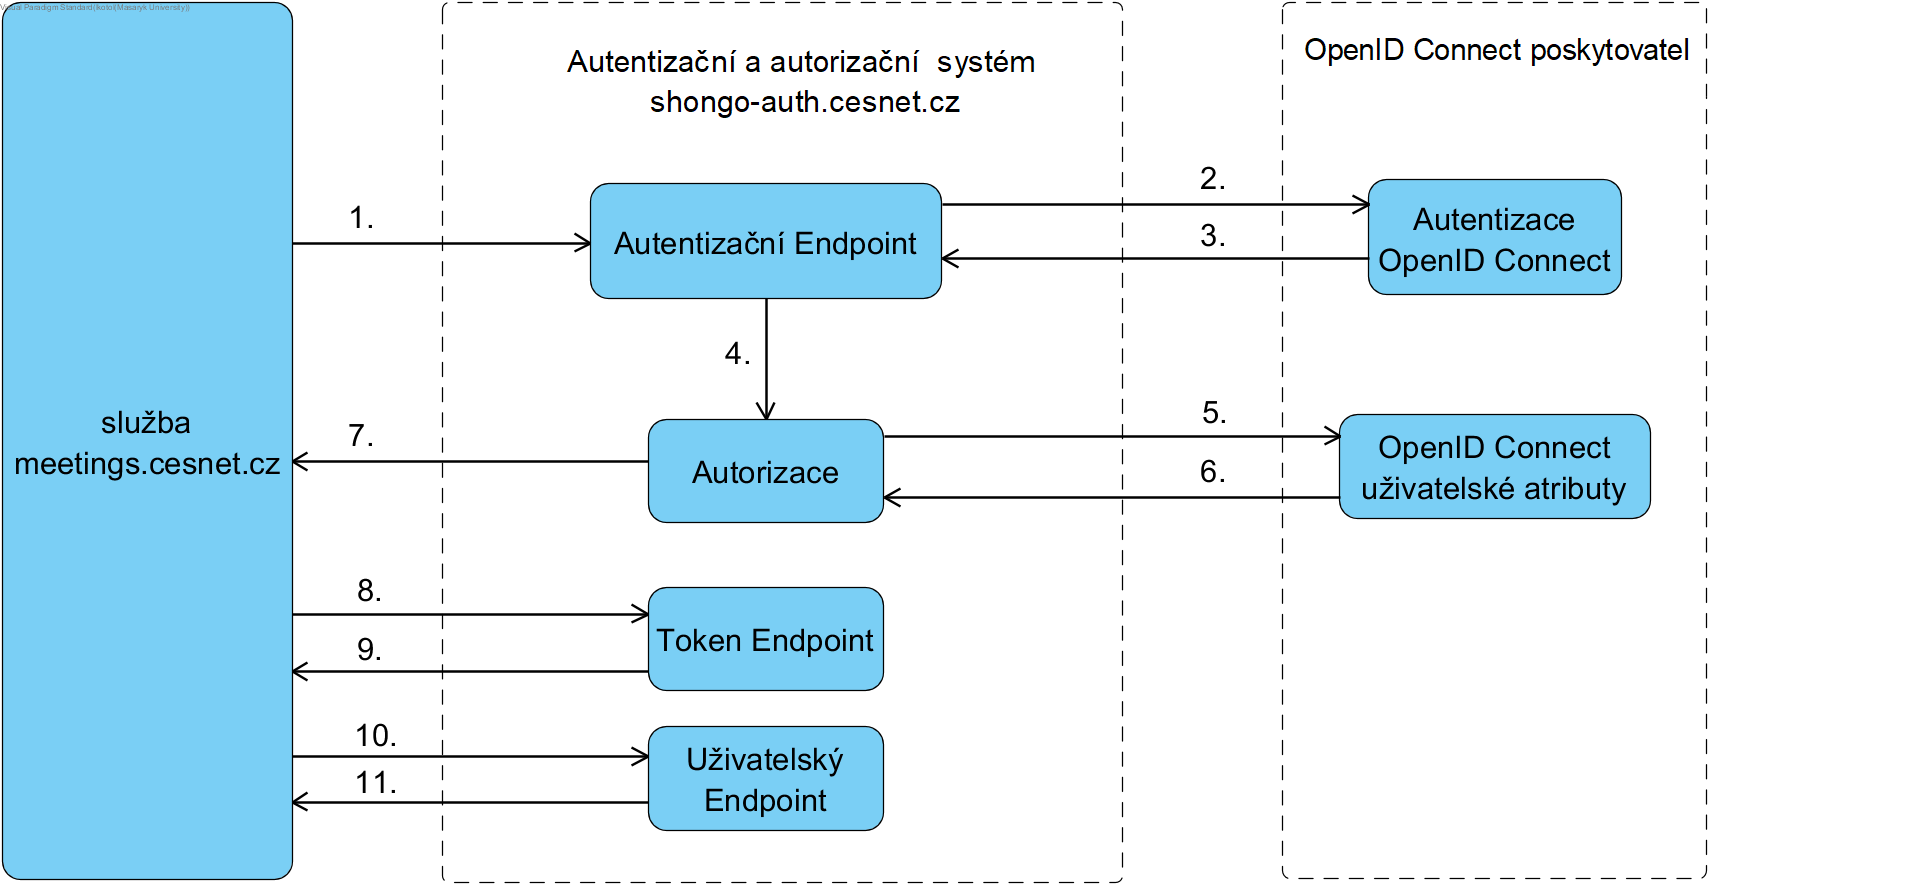
\includegraphics[width=\textwidth]{pics/meetings-oidc-obhajoba.png}
\end{frame}

\section[Zdroje]{Zdroje}

\begin{frame}[allowframebreaks]{Zdroje}
\bibliographystyle{ieeetr}
\bibliography{example}
\end{frame}


\begingroup
\setbeamercolor{background canvas}{bg=mubeamer@base}
\begin{frame}[plain]
\vfill
\centering

\includegraphics[width=\textwidth]{institution}
\vfill
\end{frame}
\endgroup

\end{document}
